\documentclass{emulateapj}

\usepackage{epsfig}
\usepackage{amsmath}
\usepackage{rotating}
\usepackage{natbib}
%\usepackage{lscape}
\usepackage{enumerate}
\usepackage{multirow}
\usepackage{array}
\usepackage{appendix}
\usepackage{comment}
\usepackage[dvipdfmx]{color}
%\usepackage[dvipdfmx]{graphicx}

\bibliographystyle{apj}

\def\memoYF#1{\color{red}$[${\bf #1}$]$ \color{black}}

\def\memoDS#1{\color{blue}$[${\bf #1}$]$ \color{black}}

\def\plotonesc#1{\centering \leavevmode
\includegraphics[clip=, width=1.70\columnwidth]{#1}}
\def\plotoneh#1{\centering \leavevmode
\includegraphics[clip=, width=.95\columnwidth]{#1}}
\def\plotone#1{\centering \leavevmode
\includegraphics[clip=, width=.85\columnwidth]{#1}}
\def\plotoneShrinkSmall#1{\centering \leavevmode
\includegraphics[clip=, width=.49\columnwidth]{#1}}
\def\plotoneShrinkMed#1{\centering \leavevmode
\includegraphics[clip=, width=.55\columnwidth]{#1}}
\def\plotoneShrinkBig#1{\centering \leavevmode
\includegraphics[clip=, width=.65\columnwidth]{#1}}
\def\plottwo#1#2{\centering \leavevmode
\includegraphics[width=.45\columnwidth]{#1} \hfil
\includegraphics[width=.45\columnwidth]{#2}}
\def\plottwob#1#2{\centering \leavevmode
\includegraphics[width=.49\columnwidth]{#1} \hfil
\includegraphics[width=.49\columnwidth]{#2}}
\def\plottwor#1#2{\centering \leavevmode
\includegraphics[width=.55\columnwidth,angle=90]{#1} \hfil
\includegraphics[width=.55\columnwidth,angle=90]{#2}}
\def\plotthree#1#2#3{\centering \leavevmode
\includegraphics[width=.3\columnwidth]{#1} \hfil
\includegraphics[width=.3\columnwidth]{#2} \hfil
\includegraphics[width=.3\columnwidth]{#3}}

\newcommand{\cN}[1]{\mathcal{N}}
\newcommand{\pn}[1]{\mbox{$(#1)$}}
\newcommand{\spa}{\mbox{ }}
\def\gsim{\;\rlap{\lower 2.5pt
 \hbox{$\sim$}}\raise 1.5pt\hbox{$>$}\;}
\def\lsim{\;\rlap{\lower 2.5pt
   \hbox{$\sim$}}\raise 1.5pt\hbox{$<$}\;}

% set formatting properties
\setlength{\textwidth}{6.5in}
\setlength{\textheight}{8.8in}
\setlength{\hoffset}{0.0in}
\setlength{\voffset}{-0.4in}
%\setlength{\voffset}{0.3in}
\parindent 0.2in
\parskip 0.1in



%%%%%%%%%%%%%%%%%%%%%%%%%%%%%%%%%%%%%%%%%%%%%%%%%
% THE DOCUMENT BEGINS HERE                      %
%%%%%%%%%%%%%%%%%%%%%%%%%%%%%%%%%%%%%%%%%%%%%%%%%

%\slugcomment{Submitted to ApJ, 20 October 2011}

\begin{document}


%%% Begin front material
%\twocolumn[%%% Begin front material

\title{Red-Giant Hot Jupiters: Brilliant Radio Emitter?}


\author{
%
Yuka Fujii\altaffilmark{0} \\
%
David S. Spiegel\altaffilmark{1, 2} \\
%
{\bf and some order:} \\
%
Jason Nordhaus\altaffilmark{3} \\
%
Nikku Madhusudhan\altaffilmark{4} \\
%
Mehrdad Mirbabayi\altaffilmark{1} \\
%
Aaron Parsons\altaffilmark{5} \\
%
Tony Mroczkowski\altaffilmark{6} \\
%
Neil Zimmerman\altaffilmark{7}
}

\affil{$^0$Earth-Life Science Institute, Tokyo Institute of Technology, 
  Tokyo, JAPAN, 152-8550}
  
\affil{$^1$Astrophysics Department, Institute for Advanced Study,
  Princeton, NJ 08540}

\affil{$^2$Research \& Development, Sum Labs,
  New York, NY  10001}

\affil{$^2$Department of Mathematics, Rochester Institute of Technology}

\affil{$^3$Astronomy Department, University of Cambridge, UK}

\affil{$^4$Astronomy Department, UC Berkeley}

\affil{$^5$Naval Research Laboratory}

\affil{$^6$Department of Mechanical and Aerospace Engineering, Princeton University, Princeton, NJ 08544}


\vspace{0.5\baselineskip}

\email{
dave@ias.edu
}


\begin{abstract}
  Red-giant hot Jupiters are jovian planets orbiting red-giant-branch
  or asymptotic-giant-branch (AGB) stars.  Post-main-sequence stars
  lose mass at much higher rates than main-sequence stars.  A jovian
  planet passing through the dense winds of its AGB host can capture
  stellar wind in its magnetosphere.  The cyclotron frequency of
  electrons from the stellar wind accreting onto the planet scales as
  100~MHz~$(B/30 {\rm~Gauss})$.  Such a planet might generate a radio
  luminosity that would be visible from kiloparsec distances.
\end{abstract}


\keywords{planets and satellites: Jupiter --- Sun: evolution ---
  planetary systems --- radiative transfer --- stars: evolution ---
  stars: AGB and post-AGB}
%]%%% End front material

%%%%%%%%%%%%%%%%%%%%%%%%%%%%%%%%%%%%%%%%%%%%%%%%%%%%%%%%%%%%%%%%%%%
\section{Introduction}
\label{sec:intro}
%%%%%%%%%%%%%%%%%%%%%%%%%%%%%%%%%%%%%%%%%%%%%%%%%%%%%%%%%%%%%%%%%%%



Planets with strong magnetic fields may generate radio or X-ray emission when interacting with energetic charged particles. 
It has been known that Jupiter emits radio emission from the radiation belt and auroral region due to the acceleration of the plasmas. \memoYF{?}. Potentially, large exoplanets can also emit radio waves through the similar mechanisms, depending on their intrinsic magnetic fields and the density of surrounding plasmas, e.g. stellar wind particles and particles from Io-like moons. 
Radio emissions from exoplanets have been estimated taking account of several possible processes, based on the empirical scaling of the radio intensity with the solar wind flux \citep{zarka2001,griebmeier2007,noyola2014}. 
Although the search for these radio signatures are being conducted, there is no clear detection claimed so far, while some indications were obtained \memoYF{?} \citep{lecavelier_et_al2013}. 
%In general, there are four proposed models for a planet to emit radio wave \citep{griebmeier2007}: 1) the magnetic energy model, 2) kinetic energy model, 3) CME model, and 4) the unipolar interaction model. 
%The search for these radio emissions from extrasolar Jovian planets has been performed. 


%It has been predicted that
% fix
When stars less than $\sim$8~$M_\sun$ evolve off the main sequence,
they go through stages on the red-giant branch (RGB) and the
asymptotic-giant branch (AGB) where their radii and luminosities increase by orders of magnitude. 
Jovian planets in orbit around such stars can be transiently heated to hot-Jupiter temperatures ($\sim$1000~K or more) at distances out to tens of AU, depending on the star's mass \citet{spiegel+madhusudhan2012}. 
At the same time, they are subject to massive stellar wind, because the mass-loss rate of such evolved stars are significantly higher than the main-sequence counterparts, typically $\sim  10^{-8} M_{\odot }$/yr \citep{judge1991}. \memoYF{How these values are observationally obtained?} \memoYF{Dave mentioned $\sim  10^{-5} M_{\odot }$/yr, where does this come from?} through massive (but slow) stellar wind \citep{suzuki2008} \memoYF{cite more papers?}. 
On the assumption that the radio emission is correlated with the stellar wind, planetary companions around evolved stars could generate bright radio emission. 

In this paper we propose the potential to detect planetary companions around evolved stars through the brightness of their radio emission. 
The search for such emission could tell us the population of companions around evolved stars, including those were originally A or O stars. 

In \S2, we discuss the assumption we make in this paper. 
\S3, we provide the estimates. 
\S4, we examine the possible obstacles to detect radio emission from the companion, taking account of the intrinsic radio emission of the evolved stars...
% based on the number of targets in the observable volumes


%Red giants lose their masses at a high rate, typically $\sim  10^{-5} M_{\odot }/yr $ through massive stellar wind. These stellar wind particle can 


%Roughly 20\% of the more than 700 \memoYF{check!} currently known exoplanets around main-sequence stars \footnote{See online catalogs such as http://www.openexoplanetcatalogue.com/ \citep{rein2012}, http://exoplanet.eu \citep{schneider_et_al2011}, or http://exoplanets.org \citep{wright_et_al2011} for up-to-date lists.} have masses greater than half of Jupiter's, orbital radii greater than 1~AU, and will become hot Jupiters (i.e., for the present purposes, this means they will receive at least as much irradiation as the currently known hot Jupiters/Neptunes \citep{spiegel+madhusudhan2012}. 


%%%%%%%%%%%%%%%%%%%%%%%%%%%%%%%%%%%%%%%%%%%%%%%%%%%%%%%%%%%%%%%%%%%
\section{Model}
\label{s:assumptions}
%%%%%%%%%%%%%%%%%%%%%%%%%%%%%%%%%%%%%%%%%%%%%%%%%%%%%%%%%%%%%%%%%%%

\subsection{Frequency of Radio Emission}

%Radio emission intensity of Solar System giant planets are empirically shown to be proportional to the kinetic energy or the magnetic energy of the solar wind,  which interacts with planetary magnetic field at the magnetic standoff cross section\citep[``radio Bode's law''; ][]{desch+kaiser1984}. 
%The detail of the mechanism of energy transport from the energy source into the radio emission. 

%\subsection{}
The peak of the auroral radio emission is around the cyclotron frequency, of the planetary magnetic field $f_{\rm cyc}$: 
%In our assumption, the frequency band width is assumed to be scaled with the cyclotron frequency, $f_{\rm cyc}$: 
%%%
\begin{eqnarray}
f_{\rm cyc} &=& \frac{eB}{2\pi m_e} \approx 25.4 {\rm~MHz} \left( \frac{B}{9.1 \rm~G} \right) \, ,
\label{eq:cyc} \\
B &=& \frac{\mu_0}{2\pi}\frac{\mathcal{M}}{R_p^3} \\
&\sim & 9.1{\rm~G} \left( \frac{\mathcal{M}}{\mathcal{M}_J} \right) \left( \frac{R_p}{R_{p, J}} \right)^{-3}. 
\end{eqnarray}
%%%
%where $\mathcal{M}_J = 1.56 \times 10^{27} \mbox{A m}^2$. 
For magnetic field strengths in the vicinity of $\sim$25-50~Gauss (G),
the cyclotron frequency will be in the range $\sim$75-150~MHz.

Note that the emission is observable from ground only when the maximum frequency is larger than the plasma frequency of the Earth's ionosphere,
%%%
\begin{equation}
f_{\rm c1}\sim 10~\mbox{MHz}
\end{equation}
%%%
{\it and} the maximum plasma frequency along the line of sight, $f_{\rm c2}$. 
At the favorable condition where the planet is in the near side of the spherical plane, the maximum plasma frequency corresponds to that in the vicinity of the planet, $f_{\rm plasma}$. Therefore, 
%%%
\begin{eqnarray}
f_{\rm c2} &=& f_{\rm plasma} = \frac{1}{2\pi} \sqrt{\frac{ne^2}{\epsilon _0 m_e}} \\
&\approx & 13{\rm~MHz} \left( \frac{a}{5~\mbox{AU}}\right)^{-1} \notag \\
&& \times \left( \frac{\dot M}{10^6 \dot M_{\odot}}\right)^{1/2} \left(\frac{v}{10^{-1} v_{\odot}}  \right)^{-1/2}
\end{eqnarray}
%%%

\subsection{Flux of Radio Emission}

The auroral radio spectral flux of exoplanets observed at the Earth, $F_{\nu}$ can be expressed by:
%Assuming $P_{\rm inp, J} = 2.1\times 10^{11}$ W \citep{griebmeier2007}, observed RGHJ radio emission at distance $l$ is
%%%
\begin{equation}
F_{\nu} = \frac{P_{\rm radio}}{\Omega l^2 \Delta f}
\end{equation}
%%%
where $P_{\rm radio}$ is the energy that is deposited as radio emission of considered frequency range, $\Omega $ is the solid angle of the emission, $l$ is the distance between the target and the Earth, and $\Delta f$ is frequency band width. 

We estimate the radio emission of exoplanets, $P_{\rm radio}$, simply by scaling the Jovian auroral radio emission, following the procedure of \citet{griebmeier2007}. 
This is based on the empirical good correlation between the radio emission intensity of Solar System giant planets and the input kinetic energy or the magnetic energy of the solar wind \citep[``radio Bode's law''; ][]{desch+kaiser1984}. 
The scaling factors depend on the properties of the stellar wind and the planetary magnetic field, which are examined in \S\ref{ss:mechanisms}, \S\ref{ss:stellarwind}, and \S\ref{ss:magneticfield}. 
%The detailed mechanism of auroral radio emission is not fully understand, 

We assume that the solid angle of the emission is same as the Jupiter's one for all of the exoplanets. In reality, the solid angles of auroral radio emission from  Jupiter, Saturn, and Earth are $\sim 1.6$, $\sim $6.3, and $\sim $3.5, respectively \citep{desch+kaiser1984}, which are on the same order and will not significantly affect our order-of-magnitude estimate of radio emission. 

The band width, $\Delta f$, is assumed to be proportional to the representative frequency of the emission, which is the cyclotron frequency, following the assumption of \citet{griebmeier2007}. 

%Therefore, assuming that the solid angle of emission is same for all of the planets \citep{??}, 
%%%
%\begin{equation}
%F_{\rm obs} = 3.76 \cdot 10^{-14}F_{\rm J, \oplus} \left( \frac{P_{\rm radio}}{P_{\rm radio,\,J}} \right) \left( \frac{l}{100\mbox{[pc]}} \right)^{-2} \left( \frac{f_{\rm cycs}}{f_{\rm cyc,\,J}} \right)^{-1}
%\end{equation}
%%%

%%%%%%%%%%%%%%%%%%%%%%%%%%%%%%%%%%%%%%%%%%%%%%%%%%%%%%%%%%%%%%%%%%%
\subsection{Assumptions for Radio Emission Scaling}
\label{ss:mechanisms}
%%%%%%%%%%%%%%%%%%%%%%%%%%%%%%%%%%%%%%%%%%%%%%%%%%%%%%%%%%%%%%%%%%%

Although the detail of the mechanism to generate planetary radio emission is not fully understood so far \memoYF{cite something?}, 
observations indicate that the total radio emission, $P_{\rm radio}$ is proportional to the input kinetic energy, $P_{\rm k,\,inp}$, or the input magnetic energy, $P_{\rm m,\,inp}$:
%%%
\begin{eqnarray}
P_{\rm radio} &\propto & P_{\rm inp} \\
P_{\rm inp,\,k} &=& n v^3 r_s ^2 \label{eq:Pinp_kin}, \\
P_{\rm inp,\,m} &=& v B_{\bot }^2 r_s ^2 \label{eq:Pinp_mag},
\end{eqnarray}
%%%
where $n$ and $v$ are density and velocity of stellar wind, respectively, $ B_{\bot }$ is the interstellar magnetic field perpendicular to the stellar wind flow, and $r_s$ is the radius of the magnetic stand-off point. 
In the case of the Solar wind, the kinetic energy is dominant input energy over the magnetic one (the former is $\sim 400$ times larger than the latter).  
It is not clear from the observations of the Solar System planets which is the fundamental one, the correlation to the input kinetic energy, that to the magnetic energy, or both. 
Because... \memoYF{I want to justify not to consider the magnetic case.}, we assume that the radio emission is scaled with the input kinetic energy, i.e., $P_{\rm radio} \propto P_{\rm k,\,inp}$. 

The radius of the magnetic stand-off point, $r_s$, is determined by the balance between the stellar wind pressure and the planetary magnetic pressure: 
%%%
\begin{eqnarray}
m_p n v ^2 &\sim& \frac{B^2}{2\pi}\left( \frac{r_s}{R_p} \right)^{-6}  \\
&=& \frac{1}{2\pi }\left( \frac{\mu _0}{2\pi } \frac{\mathcal{M}}{r_s^3} \right)^2 %\frac{B^2}{2\pi}\left( \frac{r_s}{R_p} \right)^{-6} 
\end{eqnarray}
%%%
or, 
%%%
\begin{equation}
r_s \sim \left( \frac{\mu_0^2 \mathcal{M}^2}{8\pi^3 m_{\rm p}nv^2}
\right)^{1/6}   
\end{equation}
%\begin{eqnarray}
%r_s &\sim& \left( \frac{\mu_0^2 \mathcal{M}^2}{8\pi^3 m_{\rm p}nv^2} \right)^{1/6} \\
%&=& 4.6 R_J \left( \frac{\mathcal{M}}{\mathcal{M}_J} \right)^{1/3} \left( \frac{\dot M}{\dot M_{\odot }} \right)^{-1/6} \left( \frac{v}{v_{\odot }} \right)^{-1/6}  
%\end{eqnarray}
%%%

Thus, the radio emission, $P_{\rm radio}$, or equivalently the input kinetic energy, $P_{\rm k,\,inp}$, are estimated with $n$, $v$, and $\mathcal{M}$, which should be specified by assuming the properties of the stellar wind and the planetary magnetic field. 
In the following, we describe our assumptions for these properties. 

%Thus, 
%r_s = \left[ \frac{\mu_0 f_0^2 \mathcal{M}}{8\pi^2 (m_p n(d) v(d)^2 + 2 n(d) k_B T)} \right]^{1/6}. 
%\end{equation}
%%%
%where $\mathcal{M}$ is the planetary magnetic moment and $m_p$ is the proton mass.






%%%%%%%%%%%%%%%%%%%%%%%%%%%%%%%%%%%%%%%%%%%%%%%%%%%%%%%%%%%%%%%%%%%
\subsection{Assumptions for Stellar Wind}
\label{ss:stellarwind}
%%%%%%%%%%%%%%%%%%%%%%%%%%%%%%%%%%%%%%%%%%%%%%%%%%%%%%%%%%%%%%%%%%%

The stellar wind density, $n$ in equation \ref{eq:Pinp_kin} are estimated by
%%%
\begin{equation}
n = \frac{\dot M}{4\pi a^2 m_p v}
\end{equation}
%%%
where $\dot M$ is the mass loss rate, $a$ is the orbital distance from the star and $m_p$ is proton mass. 
The mass loss rate of red giants are typically $\dot M \sim 10^{-8} M_{\odot}$/yr based on observation \memoYF{How?}. The rate can be as high as $10^{-5} M_\odot~{\rm yr^{-1}}$ during AGB phases, significantly greater than the solar mass-loss rate $\dot M_{\odot } \sim 10^{-14} M_{\odot}$/yr. 
Therefore, we have
%\memoDS{Can be as high as $10^{-5} M_\odot~{\rm yr^{-1}}$ during AGB phases.  I'm calling it ``red giant'' but we're really thinking of AGB stars for maximum mass-loss and brightness.}
\begin{equation}
\frac{\dot M}{\dot M_{\odot}} \sim 10^6 - 10^9
\end{equation}

On the other hand, the stellar wind velocity becomes smaller because of the small escape velocity (due to expanded stellar radius)\footnote{Escape velocity is $\sqrt{2GM/r}$.}. Assuming that the stellar wind scales as the escape velocity, RGs with radius $R=100R_{\odot}$ have 10 times as slow stellar wind as that at the main sequence. \memoYF{Estimate in more detail?}
\begin{equation}
\frac{v}{v_{\odot}} \sim 10^{-1}
\end{equation}

The temperature of stellar wind of RGs is expected to be 2 orders of magnitude lower than their main sequence counterparts, mainly because the sound speed of hot corona exceeds the escape speed, i.e., hot corona cannot be confined in the stellar atmosphere \citep{suzuki2008}. 
\begin{equation}
\frac{T}{T_{\odot}} \sim 10^{-2}
\end{equation}

%%%%%%%%%%%%%%%%%%%%%%%%%%%%%%%%%%%%%%%%%%%%%%%%%%%%%%%%%%%%%%%%%%%
\subsection{Assumptions for Planetary Magnetic Field}
\label{ss:magneticfield}
%%%%%%%%%%%%%%%%%%%%%%%%%%%%%%%%%%%%%%%%%%%%%%%%%%%%%%%%%%%%%%%%%%%

\memoYF{It may be better to consider Cristensen's scaling, taking account of the age. But I have not followed the theory yet.}

Theoretically, the magnetic moment of gaseous planets are expressed with the following scaling relationship \citep{griebmeier2004}:
%%%%%%%%%% 
\begin{equation}
\mathcal{M} \propto  \omega ^{\alpha } \rho_c ^{\beta } r_c^{\gamma } \sigma ^{\delta }
\end{equation}
%%%%%%%%%%
where $\omega $ is the spin angular velocity, $\rho _c$, $r_c$ and $\sigma $ are the density, the radius, and the conductivity of the ``dynamo region'' where the density is high enough for hydrogen to be metallic, respectively. 
The scaling indexes are estimated to be $\alpha \sim 1/2-1$, $\beta \sim 1/2$, $\gamma \sim 3-4$, and $\sigma \sim -1/2-0$. In this paper, we assume $\alpha =1$, $\beta =1/2$, and $r_c = 7/2$ \citep{sano1993}. \memoYF{validity?}

Unlike usual hot jupiters, RGHJs are not subject to tidal lock, as the gravitational effects of their host star does not change even if the star evolves into red giants. Without no physical insights of the typical spin rate, we simply assume that of Jupiter: $\omega = 9.925$ [hr]. 
\memoYF{Would their spin rate become higher or lower??}

In order to evaluate $\rho _c $ and $r_c$, we need a model of internal structure of gaseous planets. 
First, we assume that the planetary radius is constant at $R_p = R_{p,J}$, as the numerical calculations show that the radii of gaseous planets over the range of $0.1 R_{p, J} < M_p < 10M_{p, J}$ (with core mass less than 10\%) are converged to $0.8 R_{p, J} < R_p < 1.2R_{p, J}$ in 1 Gyr \citep{fortney2007}. 
For the density profile, we assume a polytrope gas sphere with index $n=1$, which results in:
%%%%%%%%%% 
\begin{equation}
\rho [r] = \left( \frac{\pi M_p}{4 R_p^3} \right) \frac{\sin \left[ \pi \frac{r}{R_p} \right]}{\left( \pi \frac{r}{R_p} \right)}. \label{eq:rho_r}
\end{equation}
%%%%%%%%%%
We determine the core radius $r_c$ by assuming that the hydrogen becomes metallic when $\rho (r)$ exceeds the critical density $\rho_c=700\,\mbox{kg/m}^3$. The density of the metallic core, $\rho _c$ is obtained by averaging the density in the core. 
We assume that the conductivity $\sigma $ is the same as Jupiter \memoYF{?}. 



%%%%%%%%%%%%%%%%%%%%%%%%%%%%%%%%%%%%%%%%%%%%%%%%%%%%%%%%%%%%%%%%%%%
%\subsection{Cut-off frequency}
%\label{ss:cutoff}
%%%%%%%%%%%%%%%%%%%%%%%%%%%%%%%%%%%%%%%%%%%%%%%%%%%%%%%%%%%%%%%%%%%


%%%%%%%%%%%%%%%%%%%%%%%%%%%%%%%%%%%%%%%%%%%%%%%%%%%%%%%%%%%%%%%%%%%
\section{Results}
\label{s:result}
%%%%%%%%%%%%%%%%%%%%%%%%%%%%%%%%%%%%%%%%%%%%%%%%%%%%%%%%%%%%%%%%%%%

%%%%%%%%%%%%%%%%%%%%%%%%%%%%%%%%%%%%%%%%%%%%%%%%%%%%%%%%%%%%%%%%%%%
\subsection{Estimate of Radio emission of RGHJs in comparison with canonical HJs}
%%%%%%%%%%%%%%%%%%%%%%%%%%%%%%%%%%%%%%%%%%%%%%%%%%%%%%%%%%%%%%%%%%%

On the assumption that the radio emission is proportional to the input kinetic energy (equation (\ref{eq:Pinp_kin})), the scaling of the radio emission is expanded as follows: 
%%%
\begin{eqnarray}
P_{\rm k,\,inp} &=& nv^3 r_s^2 = n v^3 \left( \frac{\mu_0^2 \mathcal{M}^2}{8\pi^3 m_{\rm p}nv^2} \right)^{1/3}  \\
&=& P_{\rm k,\,inp,\,J} \left( \frac{\mathcal{M}}{\mathcal{M}_J} \right)^{2/3} \left( \frac{a}{5.2~\mbox{AU}} \right)^{-4/3}  \notag \\
&& \times \left( \frac{\dot M}{\dot M_{\odot}} \right)^{2/3} \left( \frac{v}{v_{\odot}} \right)^{5/3} \label{eq:Pkinp}
\end{eqnarray}
%%%

It is illustrative to compare radio emission power of canonical hot jupiters and that of red giant hot jupiters. We adopt canonical values for planetary mass, orbital distance, and orbital period of each type as shown in Table \ref{tab:comp_HJ}. Then, equation (\ref{eq:Pkinp}) can be re-normalized as 
%%%
\begin{eqnarray}
P_{\rm k,\,inp} 
&\approx & 230 ~P_{\rm k,\,inp,\,J} \left( \frac{\mathcal{M}}{\mathcal{M}_J} \right)^{2/3} \left( \frac{a}{5~\mbox{AU}} \right)^{-4/3} \notag \\
&& \times \left( \frac{\dot M}{10^6 \dot M_{\odot}} \right)^{2/3} \left( \frac{v}{10^{-1} v_{\odot}} \right)^{5/3}  \\
&\approx & 2.3 \times 10^4 ~P_{\rm k,\,inp,\,J} \left( \frac{\mathcal{M}}{\mathcal{M}_J} \right)^{2/3} \left( \frac{a}{5~\mbox{AU}} \right)^{-4/3} \notag \\
&& \times \left( \frac{\dot M}{10^9 \dot M_{\odot}} \right)^{2/3} \left( \frac{v}{10^{-1} v_{\odot}} \right)^{5/3}  \\
&\approx & 100 ~P_{\rm k,\,inp,\,J} \left( \frac{\mathcal{M}}{0.1\mathcal{M}_J} \right)^{2/3} \left( \frac{a}{0.05~\mbox{AU}} \right)^{-4/3} \notag \\
&& \times \left( \frac{\dot M}{\dot M_{\odot}} \right)^{2/3} \left( \frac{v}{v_{\odot}} \right)^{5/3} 
\end{eqnarray}
%%%
\memoYF{what is the typical wind velocity of AGB stars?}
Thus, the jupiters to the AGB stars are intrinsically 200 times as bright as canonical hot Jupiters. In other words, we could search for radio signal from these stars in $(\sqrt{200})^3 \approx 3000$ times as large volume as the canonical hot jupiters.  




%%%%%%%%%%%%%%%%%%%%%%%%%%%%%%%%
\begin{table}[htdp]
\caption{Canonical Parameters of 2 types of hot jupiters.}
\begin{center}
\begin{tabular}{c|ccc} \hline \hline
& mass & orbital distance &  spin period \\ 
& $M_p$ & $a$ &  \\ \hline
canonical HJ & $M_J$ & 0.05 AU & 4 days \\
RGHJ & $M_J$ & 5 AU &  0.4 days \\ \hline
\end{tabular}
\end{center}
\label{tab:comp_HJ}
\end{table}%
%%%%%%%%%%%%%%%%%%%%%%%%%%%%%%%%



%If we consider an AGB star with mass loss rate $\dot M \sim 10^{-5} M_{\odot }\mbox{/yr}~ (=10^9 \dot M_{\odot})$, then the flux goes up to $\sim 1 \mbox{~mJy}$. 
%As the current detection limit of radio wave at $\sim 30 \mbox{~MHz}$ with Long Wavelength Array (LWA), for instance, is $\sim 1\mbox{~mJy}$ \memoYF{cite something}, this indicates that as the Sun evolves to ARB stage our Jupiter will eventually become so brilliant in radio wave that it can be detected from 100 pc away!
%\memoYF{only if $v \sim 10^{-1} v_{\odot}$. Is this validated???}
% <---- No, in this case f_plasma > 30 MHz

%%%%%%%%%%%%%%%%%%%%%%%%%%%%%%%%%%%%%%%%%%%%%%%%%%%%%%%%%%%%%%%%%%%
\subsection{Observable spectral radio emission of RGHJs with varying mass and orbital distance}
%%%%%%%%%%%%%%%%%%%%%%%%%%%%%%%%%%%%%%%%%%%%%%%%%%%%%%%%%%%%%%%%%%%


We now turn to the spectral radio flux observed at the Earth: 
%%%
\begin{eqnarray}
F_{\nu} &=& \frac{P_{\rm radio}}{\Omega d^2 f_{\rm cyclotron}} \\
%&=& P_{\rm radio,\,J} \\
&\approx & 5.4\times 10^{-6} \mbox{Jy} \left( \frac{d}{10\mbox{~pc}} \right)^{-2}  \notag \\
&&\times \left( \frac{\mathcal{M}}{\mathcal{M}_J} \right)^{-1/3}  \left( \frac{a}{5~\mbox{AU}} \right)^{-4/3} \notag \\
&& \times \left( \frac{\dot M}{\dot M_{\odot}} \right)^{2/3} \left( \frac{v}{v_{\odot}} \right)^{5/3} \\
%%%
&\approx & 1.0 \times 10^{-3} \mbox{Jy} \left( \frac{d}{10\mbox{~pc}} \right)^{-2}  \notag \\
&&\times \left( \frac{\mathcal{M}}{\mathcal{M}_J} \right)^{-1/3} \left( \frac{a}{5~\mbox{AU}} \right)^{-4/3} \notag \\ 
&& \times \left( \frac{\dot M}{10^6 \dot M_{\odot}} \right)^{2/3} \left( \frac{v}{10^{-1} v_{\odot}} \right)^{5/3} \label{eq:F_nu_RGHJ} \\
%%%
&\approx & 1.0 \times 10^{-1} \mbox{Jy} \left( \frac{d}{10\mbox{~pc}} \right)^{-2}  \notag \\
&&\times \left( \frac{\mathcal{M}}{\mathcal{M}_J} \right)^{-1/3} \left( \frac{a}{5~\mbox{AU}} \right)^{-4/3} \notag \\ 
&& \times \left( \frac{\dot M}{10^9 \dot M_{\odot}} \right)^{2/3} \left( \frac{v}{10^{-1} v_{\odot}} \right)^{5/3} \label{eq:F_nu_AGB} \\
%%%
&\approx & 4.6 \times 10^{-3} \mbox{Jy} \left( \frac{d}{10\mbox{~pc}} \right)^{-2}  \notag \\
&&\times \left( \frac{\mathcal{M}}{0.1\mathcal{M}_J} \right)^{-1/3} \left( \frac{a}{5~\mbox{AU}} \right)^{-4/3} \notag \\ 
&& \times \left( \frac{\dot M}{\dot M_{\odot}} \right)^{2/3} \left( \frac{v}{v_{\odot}} \right)^{5/3} \label{eq:F_nu_RGHJs}
%\\
%&\approx &  10^{-3} \mbox{Jy} \left( \frac{P_{\rm radio}}{200 P_{\rm radio, J}} \right) \left( \frac{l}{10\mbox{~pc}} \right)^{-2} \\
%&&\times \left( \frac{\mathcal{M}}{\mathcal{M}_J} \right)^{-1} \left( \frac{R_p}{R_{p, J}} \right)^{3}
\end{eqnarray}
%%%
Here, we used $P_{\rm radio,\,J}=2.1\times 10^{11}\mbox{~W}$ \citep{griebmeier2007} \memoYF{cite original paper!}. 
\memoYF{Spectral radio flux decreases as the magnetic moment increases. Is this true?}

Combining equation (\ref{eq:F_nu}) with the scaling relation of magnetic moment described in \S\ref{ss:magneticfield}, we estimate the spectral radio flux of planetary companions with varying masses and orbital distances as shown in Figure \ref{fig:radio}. Here we assumed that the target system is located at a distance of 10~pc from the Earth. The flux can be scaled by the distance as explicitly written in equation (\ref{eq:F_nu}). 

%The hashed regions are not observable due to the plasma cutoff at Earth's ionosphere (hashed region with vertical lines) and in the vicinity of companions (hashed region with horizontal lines). Given the stellar mass-loss rate $\dot M$ and planetary mass $M_p$, the minimum orbital distance $a$ to let radio emission escape from the target system is determined by $f_{\rm cyc} = f_{\rm plasma}$. Therefore, 
%%%
%\begin{eqnarray}
%25.4 ~\mbox{MHz} \left( \frac{\mathcal{M}}{\mathcal{M}_J} \right) &=& 12.6 ~\mbox{MHz} \left( \frac{a_{\rm min}}{5~\mbox{AU}} \right) \notag \\ 
%&& \times \left( \frac{\dot M}{10^6 \dot M_{\odot}} \right)^{1/2} \left( \frac{v}{v_{\odot}} \right)^{-1/2} \\
%\end{eqnarray}
%%%

%%%%%%%%%%%%%%%%%%%%%%%%%%%%%%%%%%%
\begin{figure*}[bp]
 \begin{minipage}{0.5\hsize}
  \begin{center}
   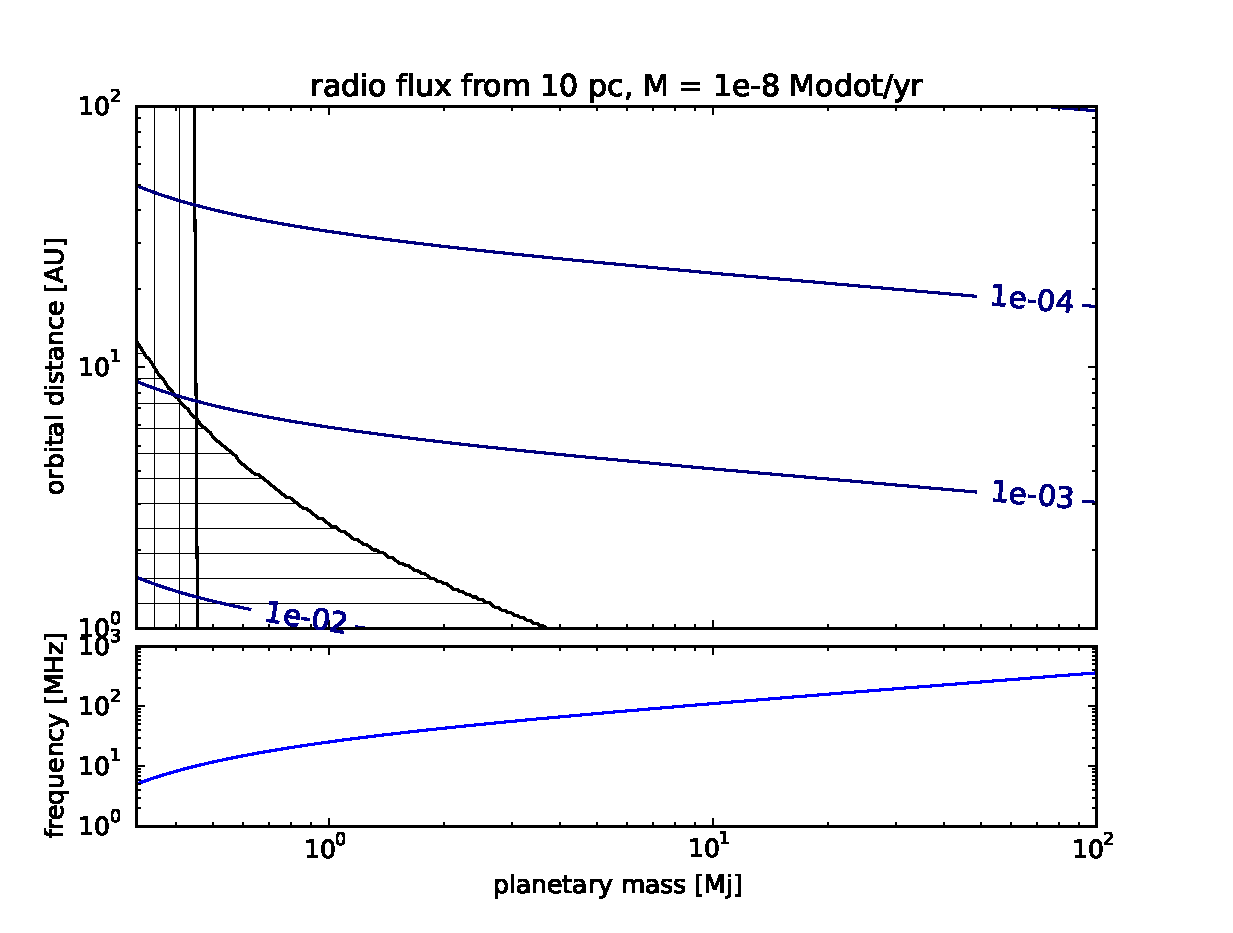
\includegraphics[width=\hsize]{radio_emission_Mdot1e-8_constRp.eps}
  \end{center}
 \end{minipage}
 \begin{minipage}{0.5\hsize}
  \begin{center}
   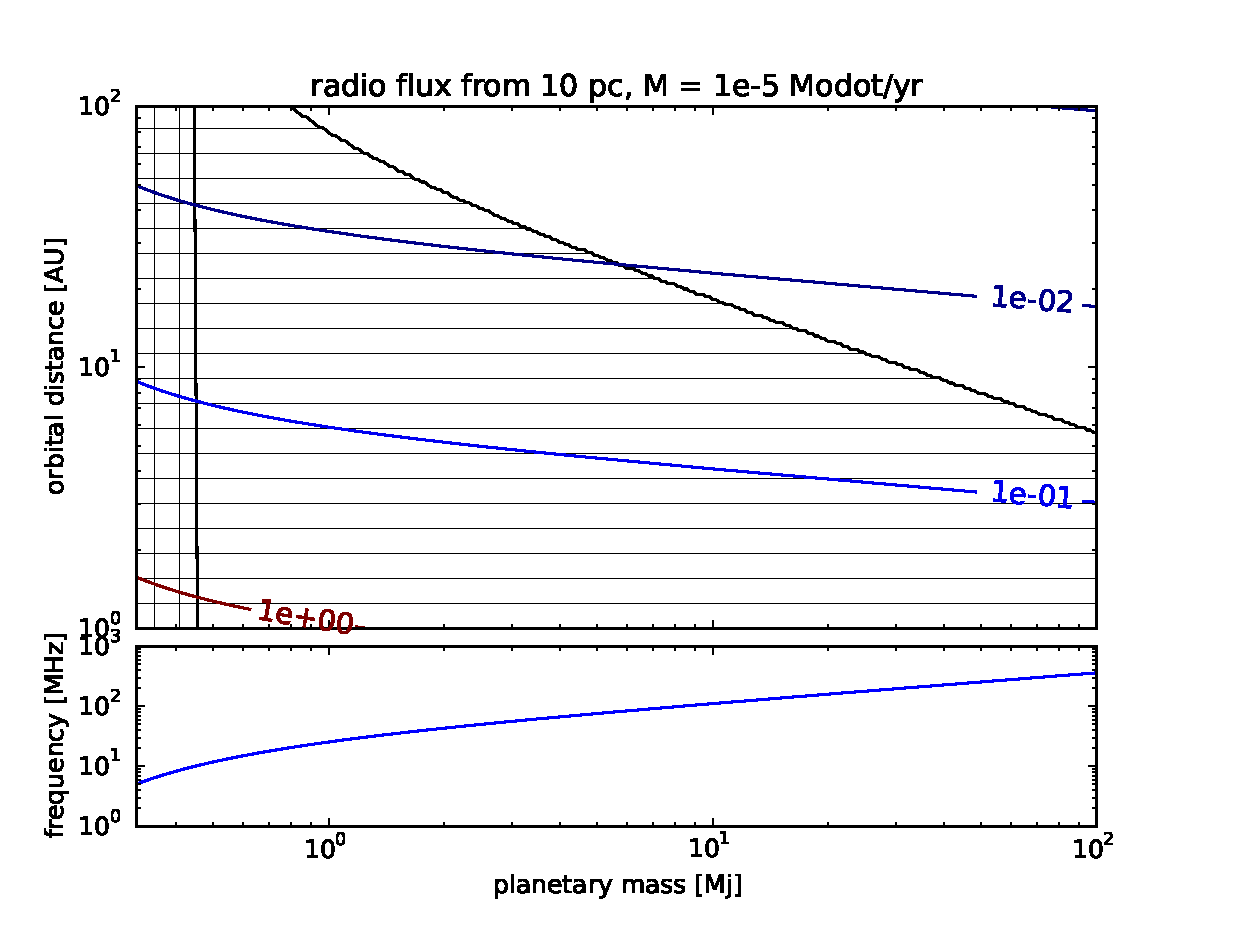
\includegraphics[width=\hsize]{radio_emission_Mdot1e-5_constRp.eps}
  \end{center} 
 \end{minipage}
   \caption{Top panel: Intensity of radio emission (in the unit of Jy) from a companion to a RG star (left) and an AGB star at 1 pc. The hashed region with vertical lines are not observable because of the plasma frequency cut-off of Earth's ionosphere. The hashed region with horizontal lines are not observable because of the plasma frequency cut-off of the stellar wind plasma in the vicinity of the companion. Bottom panel: cyclotron frequency, i.e., the frequency of radio emission. }
  \label{fig:radio}
\end{figure*}
%%%%%%%%%%%%%%%%%%%%%%%%%%%%%%%%%%% 



%%%%%%%%%%%%%%%%%%%%%%%%%%%%%%%%%%%%%%%%%%%%%%%%%%%%%%%%%%%%%%%%%%%%%%%%
\newpage

%%%%%%%%%%%%%%%%%%%%%%%%%%%%%%%%%%%%%%%%%%%%%%%%%%%%%%%%%%%%%%%%%%%
\section{Discussions}
\label{s:discussion}
%%%%%%%%%%%%%%%%%%%%%%%%%%%%%%%%%%%%%%%%%%%%%%%%%%%%%%%%%%%%%%%%%%%

%%%%%%%%%%%%%%%%%%%%%%%%%%%%%%%%%%%%%%%%%%%%%%%%%%%%%%%%%%%%%%%%%%%
\subsection{Intrinsic radio emission of red giants stars}
\label{ss:RGradio}

(Jason?)

In the radio range, the brightness source of the radio emission is Rayleigh-Jeans tail of the Planck function, i.e., $S_{\nu } = 2kT\nu^2/c^2$. Recent observations revealed that this dependence on $\nu$ ($f \propto \nu^{\alpha }$ where $\alpha $ is 2) can approximately be extended as low frequency as 1 GHz \citet{gorman2013}, presumably as a result of the wavelength dependence of the opacity (at longer wavelength we see the region further from the center of the stars) and the decreased temperature as the distance from the stars increases. 
In this paper, we simply assume that the radio emission from the red giants themselves are approximated as a black body radiation. Therefore, the flux from the giants are:
%%%
\begin{eqnarray}
f_{\star } (\nu ) &=& \frac{2R_{\star }^2 k_B T \nu^2}{c^2 d^2}  \\
&\approx & 1.4 \times 10^{-9} ~\mbox{Jy} \left( \frac{d}{100 ~\mbox{pc}} \right)^{-2} \\
&& \times \left( \frac{R_{\star }}{10 R_{\odot }} \right)^2 \left( \frac{T_{\star }}{10^{4}~\mbox{K}} \right) \left( \frac{\nu}{1 ~\mbox{GHz}} \right)^2 
\end{eqnarray}
%%%
Therefore, for stars with $R_{\star } < 50 R_{\odot}$, companions around the stars are typically brighter than their hosts. 




%%%%%%%%%%%%%%%%%%%%%%%%%%%%%%%%%%%%%%%%%%%%%%%%%%%%%%%%%%%%%%%%%%%
\subsection{Will the electron spiraling and offset the magnetic field? (Mehrdad Mirababayi)}
\label{ss:offset}


\citet{gorman2013}

%%%%%%%%%%%%%%%%%%%%%%%%%%%%%%%%%%%%%%%%%%%%%%%%%%%%%%%%%%%%%%%%%%%
\subsection{Expected population of RGHJ in the observable volume}
\label{ss:number}

\newpage


\section{Dave's sketch}

\citep{spiegel2008}

\citep{lecavelier_et_al2013}

\citep{janhunen_et_al2003}

\citep{zarka1992, zarka1998}

\citep{farrell_et_al2004}

\citep{lazio+farrell2007}: likelihood function, tau Boo search

\citep{lecavelier_et_al2009}

\citep{spiegel2012}

\citep{nordhaus+spiegel2013}



\citep{jiang+jin1996}: 12cm radio of Jupiter during Shoemake-Levy-9

\citep{morin2012, morin_et_al2013}

\citep{christensen_et_al2009, christensen2010}

\citep{saar2001}: Inverse rossby number scaling of magnetic field: $B
\sim 60 {\rm~G} \times Ro^{-1.2}$.  Here, he takes $Ro = \tau_c/P_{\rm
  rot}$, where $\tau_c$ is the convective turnover time = ?
\citep{gilliland1986}.  Well, $F \sim \rho v_c^3 \sim \rho
(H/\tau_c)^3$, so $\tau_c \sim H (\rho / F)^{1/3} = H / (\sigma T_{\rm
  eff}^4 / \rho)^{1/3}$.  Alternatively, $\tau_{\rm conv} \sim (M R^2
/ L)^{1/3}$.

On dimensional grounds, the convective turnover time goes as
$\tau_{\rm conv} \sim (M R^2 / L)^{1/3}$.  According to
\citet{burrows_et_al2001}, radius $R$ and luminosity scale with time
as $R \sim R_J$, where $R_J$ is the radius of Jupiter, and
\begin{equation}
\frac{L}{10^{-9} L_\odot} \sim \left( \frac{t}{1 \rm~Gyr} \right)^{-1.3} \left( \frac{M}{1~M_J} \right)^{2.64} \, .
\label{eq:burrowsLum}
\end{equation}
So,
%\begin{eqnarray}
%\nonumber \tau_{\rm conv} & \sim & 3 {\rm~days} \times \left( \frac{M}{M_J} \right)^{1/3} \left( \frac{R}{R_J} \right)^{2/3} \left( \frac{L}{L_\odot} \right)^{-1/3} \\
% & = & 
%\end{eqnarray}
\begin{eqnarray}
\nonumber \tau_c & \sim & 3 {\rm~hrs} \times \frac{\left( \frac{H}{100 \rm~km} \right) \left( \frac{\rho}{10^{-5} \rm~g~cm^{-3}} \right)^{1/3}}{\left( \frac{L}{10^{-9} L_\odot} \right)^{1/3}} \\
 & = & 3 {\rm~hrs} \times \frac{\left( \frac{H}{100 \rm~km} \right) \left( \frac{\rho}{10^{-5} \rm~g~cm^{-3}} \right)^{1/3}}{\left( \frac{M}{1 ~M_J} \right)^{0.88} \left( \frac{t}{1 \rm~Gyr} \right)^{0.43}} \\
\end{eqnarray}
So the Rossby number $Ro = \tau_c/P_{\rm rot}$ is
\begin{eqnarray}
Ro & = & \frac{\tau_c}{P_{\rm rot}} \\
 & = & \left( \frac{P_{\rm rot}}{3 \rm~hrs} \right)^{-1} \times \frac{\left( \frac{H}{100 \rm~km} \right) \left( \frac{\rho}{10^{-5} \rm~g~cm^{-3}} \right)^{1/3}}{\left( \frac{M}{1 ~M_J} \right)^{0.88} \left( \frac{t}{1 \rm~Gyr} \right)^{0.43}}
\end{eqnarray}

\citep{hallinan_et_al2013}

\citep{desch+kaiser1984} radiometric Bode's law

Noting that
\begin{equation}
\dot{M}_* = 4\pi r^2 \rho[r] v \, ,
\label{eq:mdot
}\end{equation}
so $\rho[r] = \dot{M}_*/(4\pi r^2 v)$,
\begin{eqnarray}
\frac{\rho v^2}{2} = \frac{B^2}{8\pi} \sim \frac{B_0^2}{8\pi} \left( \frac{d}{d_0} \right)^{-3} \, ,
\end{eqnarray}
where $B_0$ is the field strength at a distance $d_0$ from the planet.
\begin{eqnarray}
\frac{\rho v^2}{2} & \sim & \frac{B_0^2}{8\pi} \left( \frac{d}{d_0} \right)^{-6} \\
\frac{\dot{M}_* v}{8\pi a^2} & = & \frac{B_0^2}{8\pi} \left( \frac{d}{d_0} \right)^{-6} \\
\frac{\dot{M}_* v}{r^2} & = & B_0^2 \left( \frac{d}{d_0} \right)^{-6} \\
d^6 & = & \frac{d_0^6 B_0^2 r^2}{\dot{M}_* v} \\
d_A & = & d_0 \left( \frac{B_0^2 r^2}{\dot{M}_* v} \right)^{1/6} \\
  & \sim & 4 R_J \left( \frac{d_0}{R_J}\right) \left\{ \frac{\left( \frac{B}{10 \rm~G} \right)^2 \left( \frac{r}{5 \rm~AU} \right)^2}{\left( \frac{\dot{M}_*}{10^{-6} M_\odot/\rm yr} \right) \left( \frac{v}{20 \rm~km/s} \right)} \right\}^{1/6}
\label{eq:Chapman-Ferraro}
\end{eqnarray}
In the above, $d_A$ is the distance from the planet to the Alfven
point, where the magnetic energy density $u_B = B^2 / 8\pi$ equals the
kinetic energy density in the stellar wind $u_w = \rho v^2/2$, and
$B_0$ is the magnetic field strength at distance $d_0$.

The escape speed is
\begin{equation}
v_{\rm esc}^* = \sqrt{\frac{2 G M_*}{R_*}} \, ,
\end{equation}
so if the stellar wind speed is a factor $C$ times the escape speed, then ...

The power incident on the planet within $d_A$ is
\begin{eqnarray}
P_{\rm inc} & = & \frac{\rho v^3}{2} \times \pi d_A^2 \\
\frac{\rho v^2}{2} & \sim & \frac{B_0^2}{8\pi} \left( \frac{d}{d_0} \right)^{-6} \\
d_A^6 & = & d_0^6 \frac{B_0^2}{4\pi \rho v^2} \\
d_A^2 & = & d_0^2 \left( \frac{B_0^2}{4\pi \rho v^2}\right)^{1/3} \\
\pi d_A^2 \frac{\rho v^3}{2} & = & \frac{d_0^2}{2} \left( \frac{\pi^2 \rho^2 v^7 B_0^2}{4} \right)^{1/3} \\
P_{\rm inc} & = & d_0^2 \left( \frac{\pi^2 \rho^2 v^7 B_0^2}{32} \right)^{1/3} 
%\frac{\dot{M}_* v}{8\pi a^2} & = & \frac{B_0^2}{8\pi} \left( \frac{d}{d_0} \right)^{-6} \\
%\frac{\dot{M}_* v}{r^2} & = & B_0^2 \left( \frac{d}{d_0} \right)^{-6} \\
%d^6 & = & \frac{d_0^6 B_0^2 r^2}{\dot{M}_* v} \\
%d_A & = & d_0 \left( \frac{B_0^2 r^2}{\dot{M}_* v} \right)^{1/6} \\
%  & \sim & 4 d_0 \left\{ \frac{\left( \frac{B}{10 \rm~G} \right)^2 \left( \frac{r}{5 \rm~AU} \right)^2}{\left( \frac{\dot{M}_*}{10^{-6} M_\odot/\rm yr} \right) \left( \frac{v}{20 \rm~km/s} \right)} \right\}^{1/6}
\end{eqnarray}
Note that $\rho v = \dot{M}_*/4\pi r^2$.  Therefore,
\begin{eqnarray}
P_{\rm inc} & = & d_0^2 \left( \frac{\pi^2 \rho^2 v^7 B_0^2}{32} \right)^{1/3} \\
 & = & d_0^2 \left( \frac{\dot{M}_*^2 v^5 B_0^2}{512 r^4} \right)^{1/3} \\
 & = & \frac{d_0^2}{8} \left( \frac{\dot{M}_*^2 v^5 B_0^2}{r^4} \right)^{1/3} \\
\nonumber  & \sim & 2 \times 10^{18} {\rm~W} \left( \frac{d_0}{R_J} \right)^2 \left( \frac{\dot{M}_*}{10^{-5} M_\odot / {\rm yr}} \right)^2 \\
 & & \times \left( \frac{v}{20 \rm~km/s} \right)^5 \left( \frac{B_0}{10 \rm~G} \right)^2 \left( \frac{r}{5 \rm~AU} \right)^{-4}
\end{eqnarray}


The power incident on the planet is

%\citep{lunine_et_al1989} -- error?

% http://kiss.caltech.edu/workshops/magnetic2013/presentations/winterhalter.pdf

%ftp://ftp.iwf.oeaw.ac.at/pub/Scherf/PRE-CD%20V2/pre6/nigl.pdf


%%%%%%%%%%%%%%%%%%%%%%%%%%%%%%%%%%%%%
\subsection{}

%%%%%%%%%%%%%%%%%%%%%%%%%%%%%%%%%%%%%%%%%%%%%%%%%%%%%%%%%%%%%%%%%%%%%%%%
\section{Conclusions}
\label{sec:conc}

\vspace{0.5in}

%\acknowledgements

{\sc Acknowledgments}

We thank many people for useful discussions, in particular Tony
Mroczkowzki.  DSS gratefully acknowledges support from a fellowship
from the AMIAS group.  NM acknowledges support from [???].

\newpage

mehrdad

\newpage

\bibliography{biblio.bib}


\clearpage

\end{document}
